\begin{figure}[H]
    \centering
    \begin{subfigure}{0.98\textwidth} 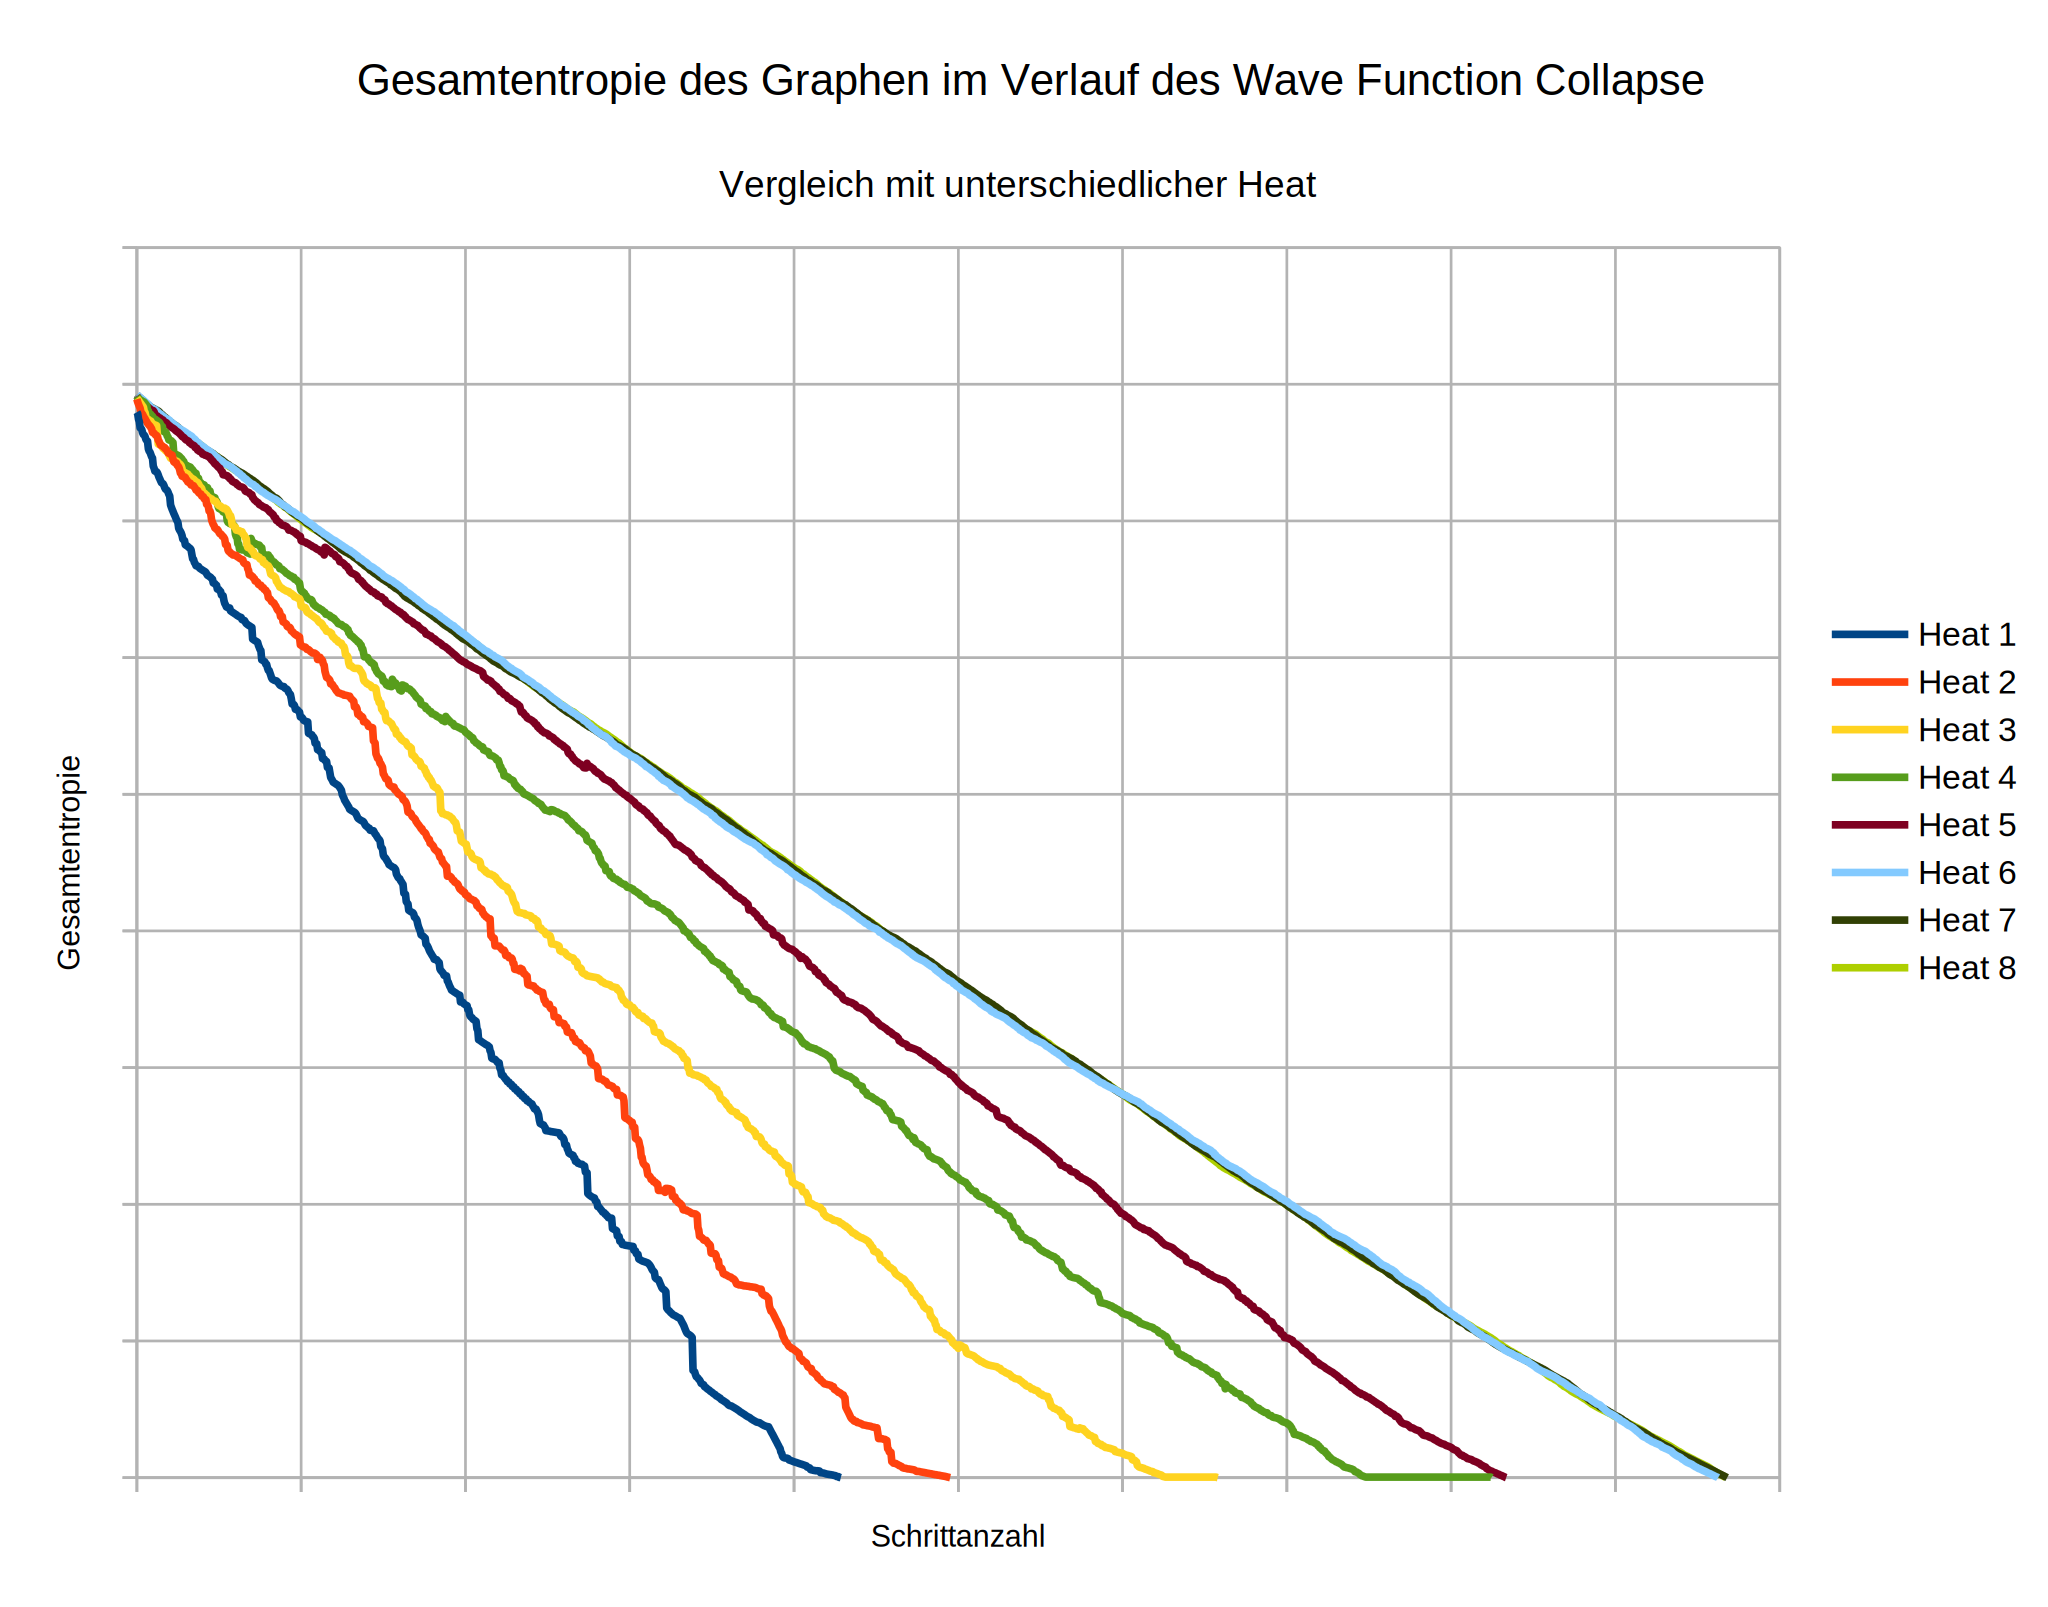
\includegraphics[width=\linewidth]{data/app/1.png}  \caption{} \end{subfigure}
    
    \caption{
        Screenshot von der Anwendung. Oben-Links sind Beispiele zur Auswahl aufgelistet und Wrapping kann eingestellt werden. Mitte-Links kann der Graph generiert werden. Und Unten-Links kann Heat eingestellt werden und der Wave Function Collapse kann gestartet/neugestartet. Man kann auch zu vorherigen Schritte zurückspulen um diese genauer zu betrachten. Auf der rechten Seite sind Menüs mit ein paar Informationen und Einstellungen um andere Daten anzuzeigen oder auszublenden.
    }
    \label{fig:app}
\end{figure}